%%%%%%%%%%%%%%%%%%%%%%%%%%%%%%%%%%%%%%%%%%%%%%%%%%%%%%%%%%%%%%%%%%%%%%%%%%


% abnTeX2: Modelo de Trabalho Acadêmico em conformidade com 
% as normas da ABNT


%%%%%%%%%%%%%%%%%%%%%%%%%%%%%%%%%%%%%%%%%%%%%%%%%%%%%%%%%%%%%%%%%%%%%%%%%%


\documentclass[english, 
               brazil, 
               bsc] %Opções bsc (TCC) e msc (Mestrado)
               {dcomp-abntex2}




%%%%%%%%%%%%%%%%%%%%%%%%%%%%%%%%%%%%%%%%%%%%%%%%%%%%%%%%%%%%%%%%%%%%%%%%%%
% Área para adição de pacotes extras
%%%%%%%%%%%%%%%%%%%%%%%%%%%%%%%%%%%%%%%%%%%%%%%%%%%%%%%%%%%%%%%%%%%%%%%%%%


% \usepackage{lipsum} % Retirar para a versão final do documento
\usepackage{float}
\usepackage{pgfgantt}
\usepackage{lscape}


\restylefloat{table}


%Utilize aqui seu pacote preferido para algoritmos
\usepackage[linesnumbered]{algorithm2e}


%%%%%%%%%%%%%%%%%%%%%%%%%%%%%%%%%%%%%%%%%%%%%%%%%%%%%%%%%%%%%%%%%%%%%%%%%%


%Compila o índice
\makeindex


\begin{document}


% Seleciona o idioma do documento (conforme pacotes do babel)
\selectlanguage{brazil}


% Retira espaço extra obsoleto entre as frases.
\frenchspacing 


%%%%%%%%%%%%%%%%%%%%%%%%%%%%%%%%%%%%%%%%%%%%%%%%%%%%%%%%%%%%%%%%%%%%%%%%%%
% ELEMENTOS PRÉ-TEXTUAIS
%%%%%%%%%%%%%%%%%%%%%%%%%%%%%%%%%%%%%%%%%%%%%%%%%%%%%%%%%%%%%%%%%%%%%%%%%%


\pretextual




\titulo{PreOCR - Trabalho de Processamento de Imagens T01 2023.2} 
\autor{Grupo 13 - Everton Santos de Andrade Júnior}
\orientador{}
\coorientador{}


% \inserirInformacoesPDF





% \inserirInformacoesPDF
%
%
\imprimircapa
% \imprimirfolhaderosto*
%  
%     
\mostrarSUMARIO


%%%%%%%%%%%%%%%%%%%%%%%%%%%%%%%%%%%%%%%%%%%%%%%%%%%%%%%%%%%%%%%%%%%%%%%%%%
% ELEMENTOS TEXTUAIS
%%%%%%%%%%%%%%%%%%%%%%%%%%%%%%%%%%%%%%%%%%%%%%%%%%%%%%%%%%%%%%%%%%%%%%%%%%


\textual


%%%%%%%%%%%%%%%%%%%%%%%%%%%%%%%%%%%%%%%%%%%%%%%%%%%%%%%%%%%%%%%%%%%%%%%%%%
% Introdução
%%%%%%%%%%%%%%%%%%%%%%%%%%%%%%%%%%%%%%%%%%%%%%%%%%%%%%%%%%%%%%%%%%%%%%%%%%
\chapter{Introdução e Resultados} \label{introduction}

Neste trabalho, desenvolvemos um programa capaz de processar imagens binárias no formato PBM ASCII (PGM tipo P1), contendo texto dos tipos e tamanhos de fontes, variando de 10 à 40. Conseguimos determinar o básico do trabalho que são o número de linhas e palavras no texto e os retangulos dessas palavras, gerando uma imagem de saída com esses retangulos. Além disso, nosso grupo implementou mais funcionalidades, como a detecção de colunas e blocos do texto, utilizando o conceito de distância alinhada. Includingo a \textit{bouding box} (bbox) desses blocos e linhas que indicam as colunas.

Adicionalmente, para ilustrar nossos resultados de forma mais interativa, geramos uma série de imagens intermediárias que mostram o processo de detecção de blocos, colunas, palavras, e linhas destacando as regiões por um retangulo de diferentes cores. O formato dessas imagems é P3 (ascii RGB).
Essas imagens foram usadas em sequencia de frames para gerar um video de saíoda usando o programa de linha de commando ``ffmpeg``.

A nossa abordagem é dinamica, baseado na altura das palavras mudamos os parametros enquanto o programa roda. Desse modo é possivel identificar estruturas de texto em diferentes alinhamentos, como justificado, esquerda, centro e direita, além de lidar com diferentes tamanhos e estilos de fonte, incluindo Comic Sans, Impact, Cascadia Code, Arial e Times New Roman. Um exemplo de video gerado pode ser encontrado em \url{https://youtu.be/uA45GeodGss?si=ZOgsA2av7EKZeG69}.

\section{Resultados}

Os resultados desse projeto podem ser bem entendidos pelas imagens coloridas geradas. . No capitulo com os detalhes das implementações. Na \autoref{cascadia} temo o resultado gerado no projeto para a entrada de um texto na fonte Cascadia Code em negrito de tamanho 10, alinhado à esquerda. Essa imagem tem baixa resolução e vem com ruídos. Mesmo assim o nosso trabalho conseguiu identificar as bbxoes das palavras, mesmo quando as letras possuvem alturas diferentes. Os retangulos em vermelho indicam essas bboxes das palavras encontradas. A linha em amarelo é feita pelo algortimo todas vez que encontra o começo de  uma coluna. Em verde está o agrupamento dos blocos ou paragrafos que o nosso trabalho conseguiu encontrar. Especificamente para essa entrada, o algoritmo encontrou 5 blocos, 2 colunas, 42 linhas e 395 palavras. Com a mesma fonte mas de tamanha 16, e centralizado, temos outro resultado na \autoref{cascadia16}, nesse encontramos 2 colunas, 4 blocos, 38 linhas e 226 palavras. Na \autoref{timesnewroman}, ja mudamos a fonte para Time News Roman, e ainda está em itálico. Nesse entrada já pulamos para quartro colunas e tamanho 18 de fonte. No resultado foi encontrado 4 colunas, 6 blocos, 38 linhas e 197 palavras. O correto deveria ser 196 palavras, o restante está correto. Pulamos para uma nova fonte chamada Impact de tamanho 40, que é um grande salto dos outros casos. Neste, o algortimo encontra 2 colunas, 2 blocos, 18 linhas e palavras 47 palavras. O correto deveria ser 46 palavras, o restante está correto. Também foi testados com fonte Arial, com exemplos tanto providos pela professor Beatriz, quanto criados pelo grupo. Um exemplo desses resultados pode ser ilutrado pela \autoref{arial}, nesse o texto é justificado com 3 colunas e tamanho 12. O algortimo encontrou tudo corretamente, com 557 palavras e 52 linhas. Por fim, demos upload da coleção de videos gerados por este trabalho com  diferentes fontes e tamanhos testados que pode ser encontrado no youtube neste link: \url{https://www.youtube.com/watch?v=uA45GeodGss}.

\begin{figure}[H]
        \caption{\label{cascadia} \small Cacadia Code em negrito, com 10 de tamanho, 2 colunas e 5 blocos de texto. A entrada possue baixa resolução e ruídos. }
        \begin{center}
            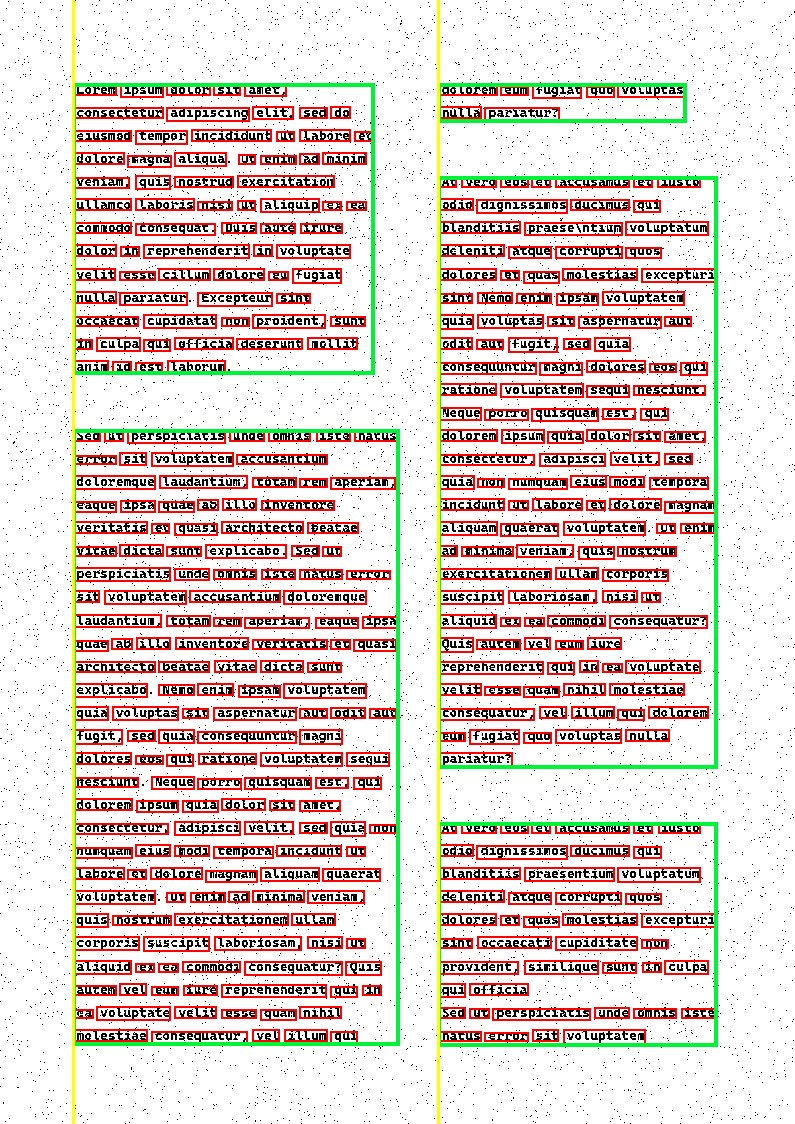
\includegraphics[scale=0.55]{./images/cascadia_code_10_detected_colunas_2_blocos_5_linhas_42_palavras_395.png}
        \end{center}
  \legend{ \small Fonte: Autor.}
\end{figure}

\begin{figure}[H]
        \caption{\label{cascadia16} \small Cacadia Code centralizado, com 16 de tamanho, 2 colunas e 4 blocos de texto. }
        \begin{center}
            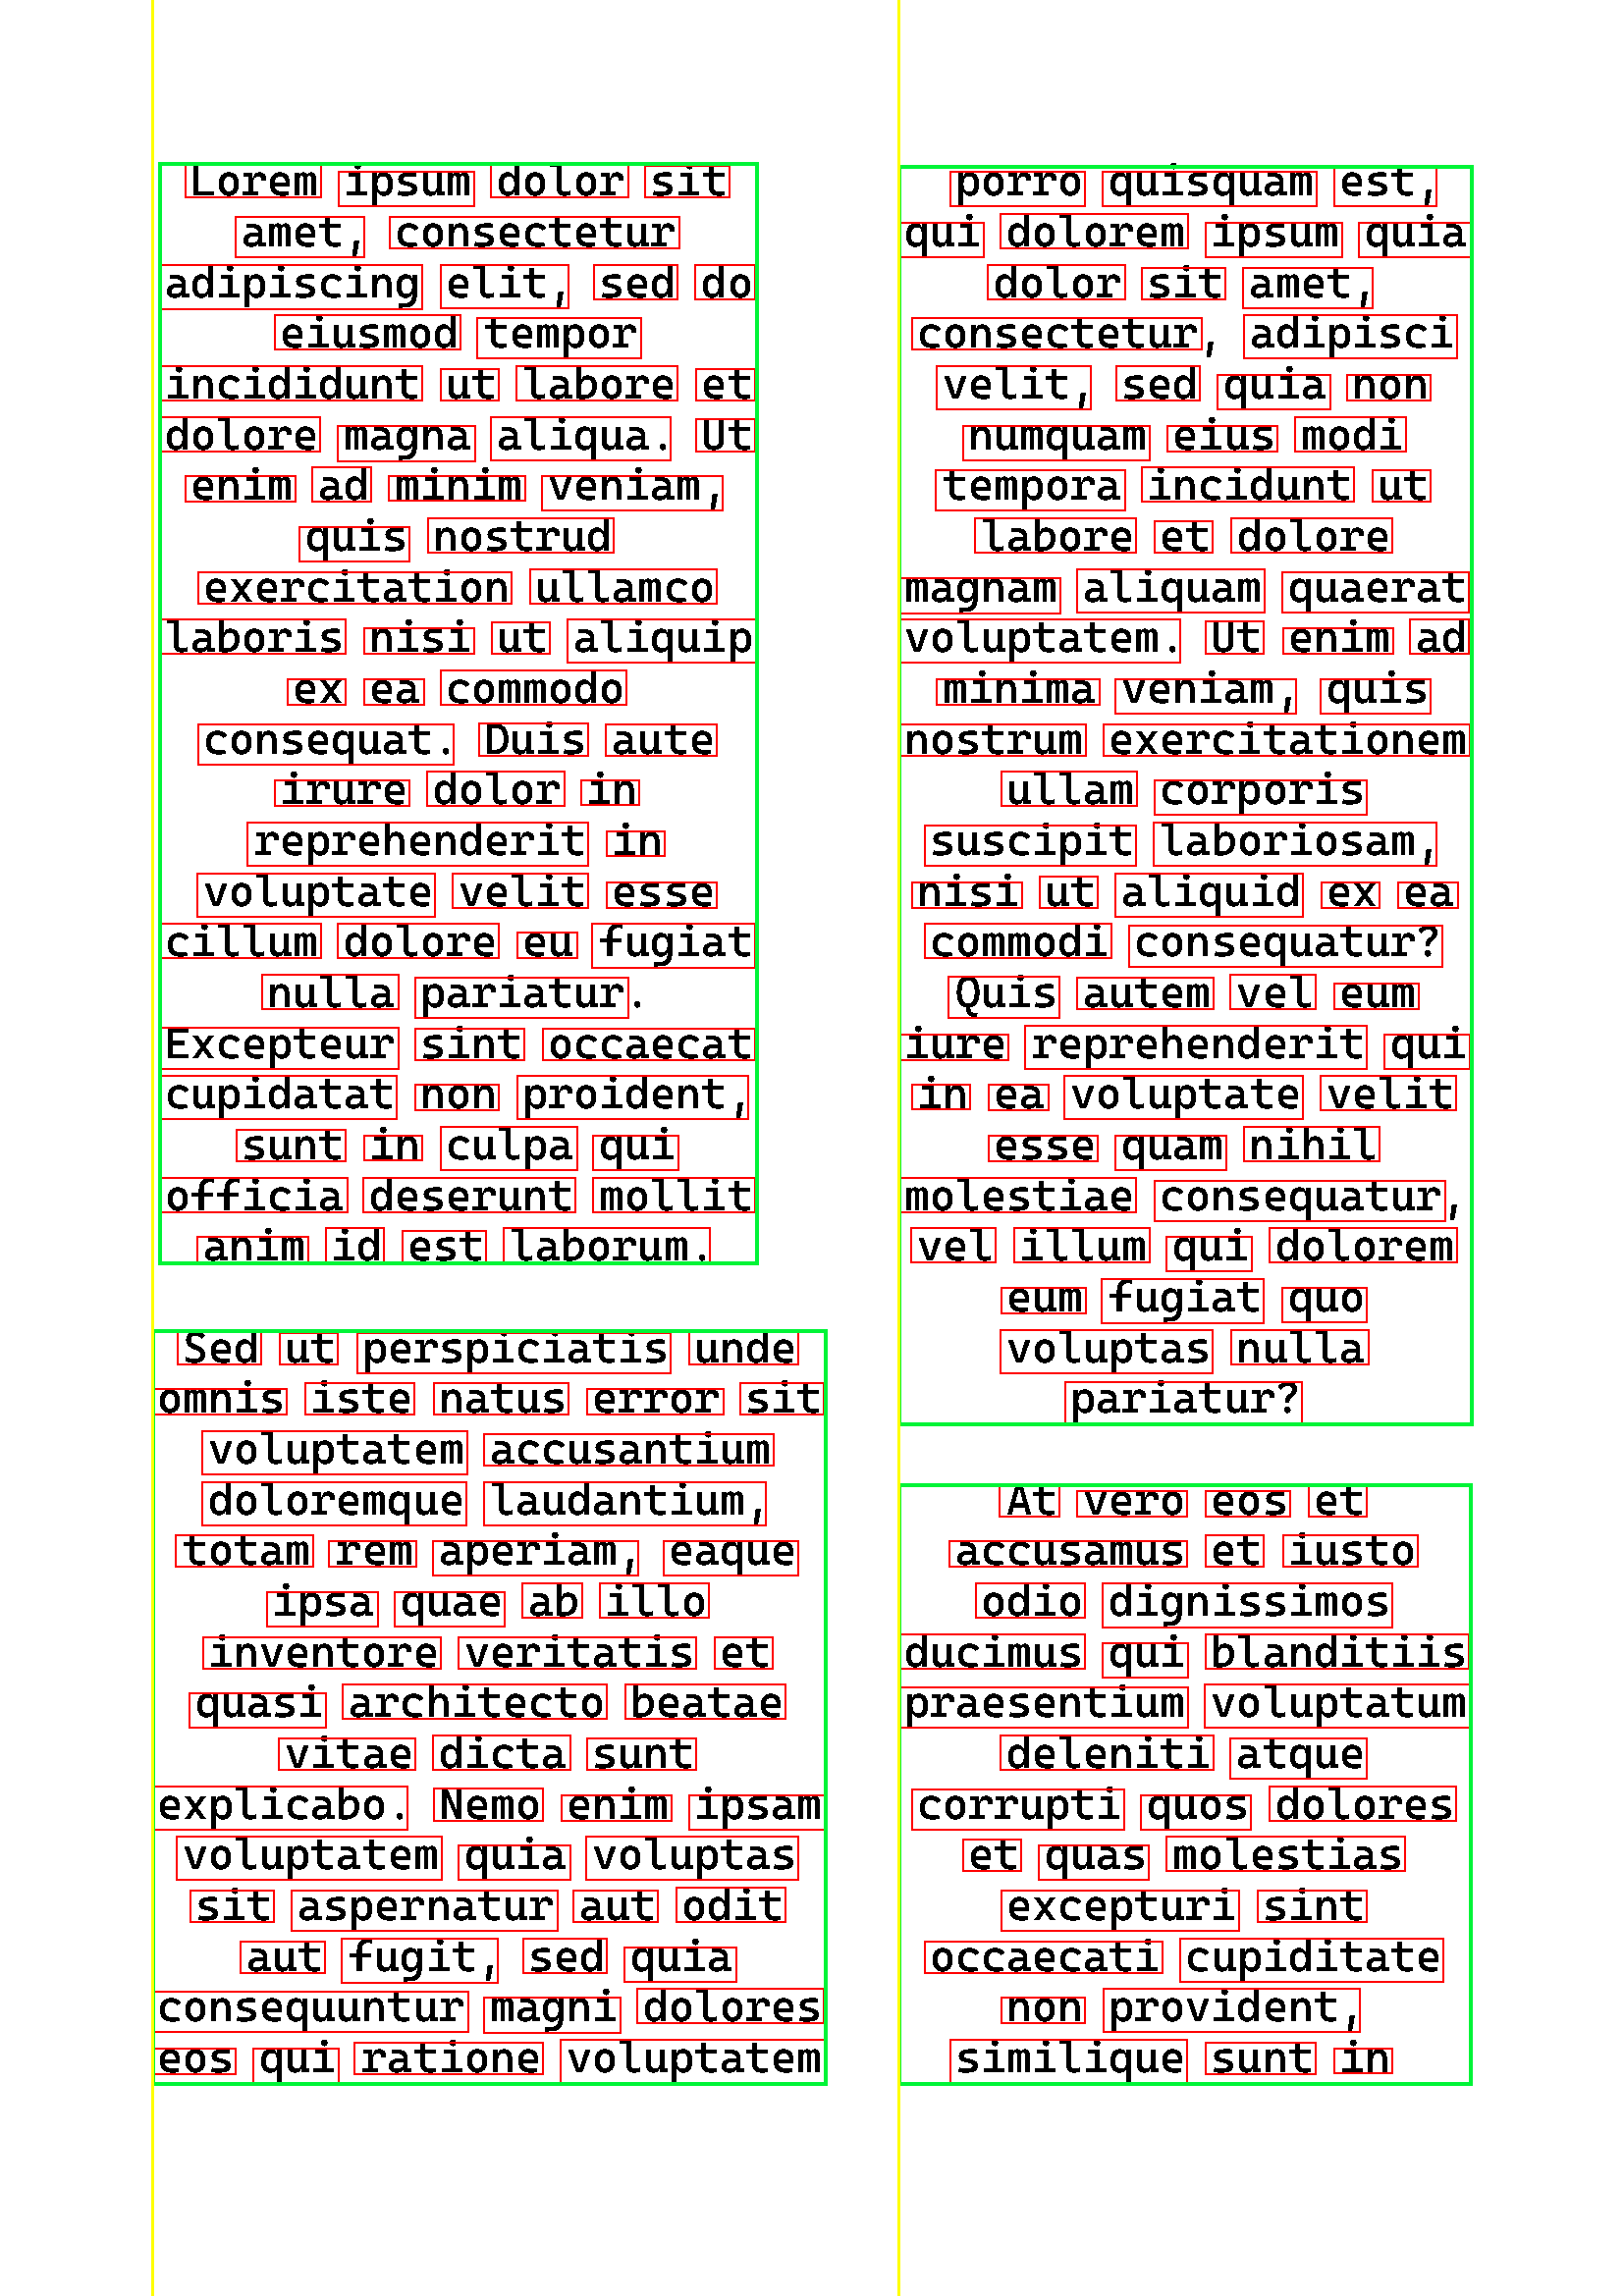
\includegraphics[scale=0.55]{./images/cascadia_code_centralizado_tamanho_16_colunas_2_blocos_4_linhas_38_palavras_226.png}
        \end{center}
  \legend{ \small Fonte: Autor.}
\end{figure}

\begin{figure}[H]
        \caption{\label{timesnewroman} \small Times News Roman em itálico, com 18 de tamanho, com 4 colunas, 6 blocos de texto.}
        \begin{center}
        \end{center}
        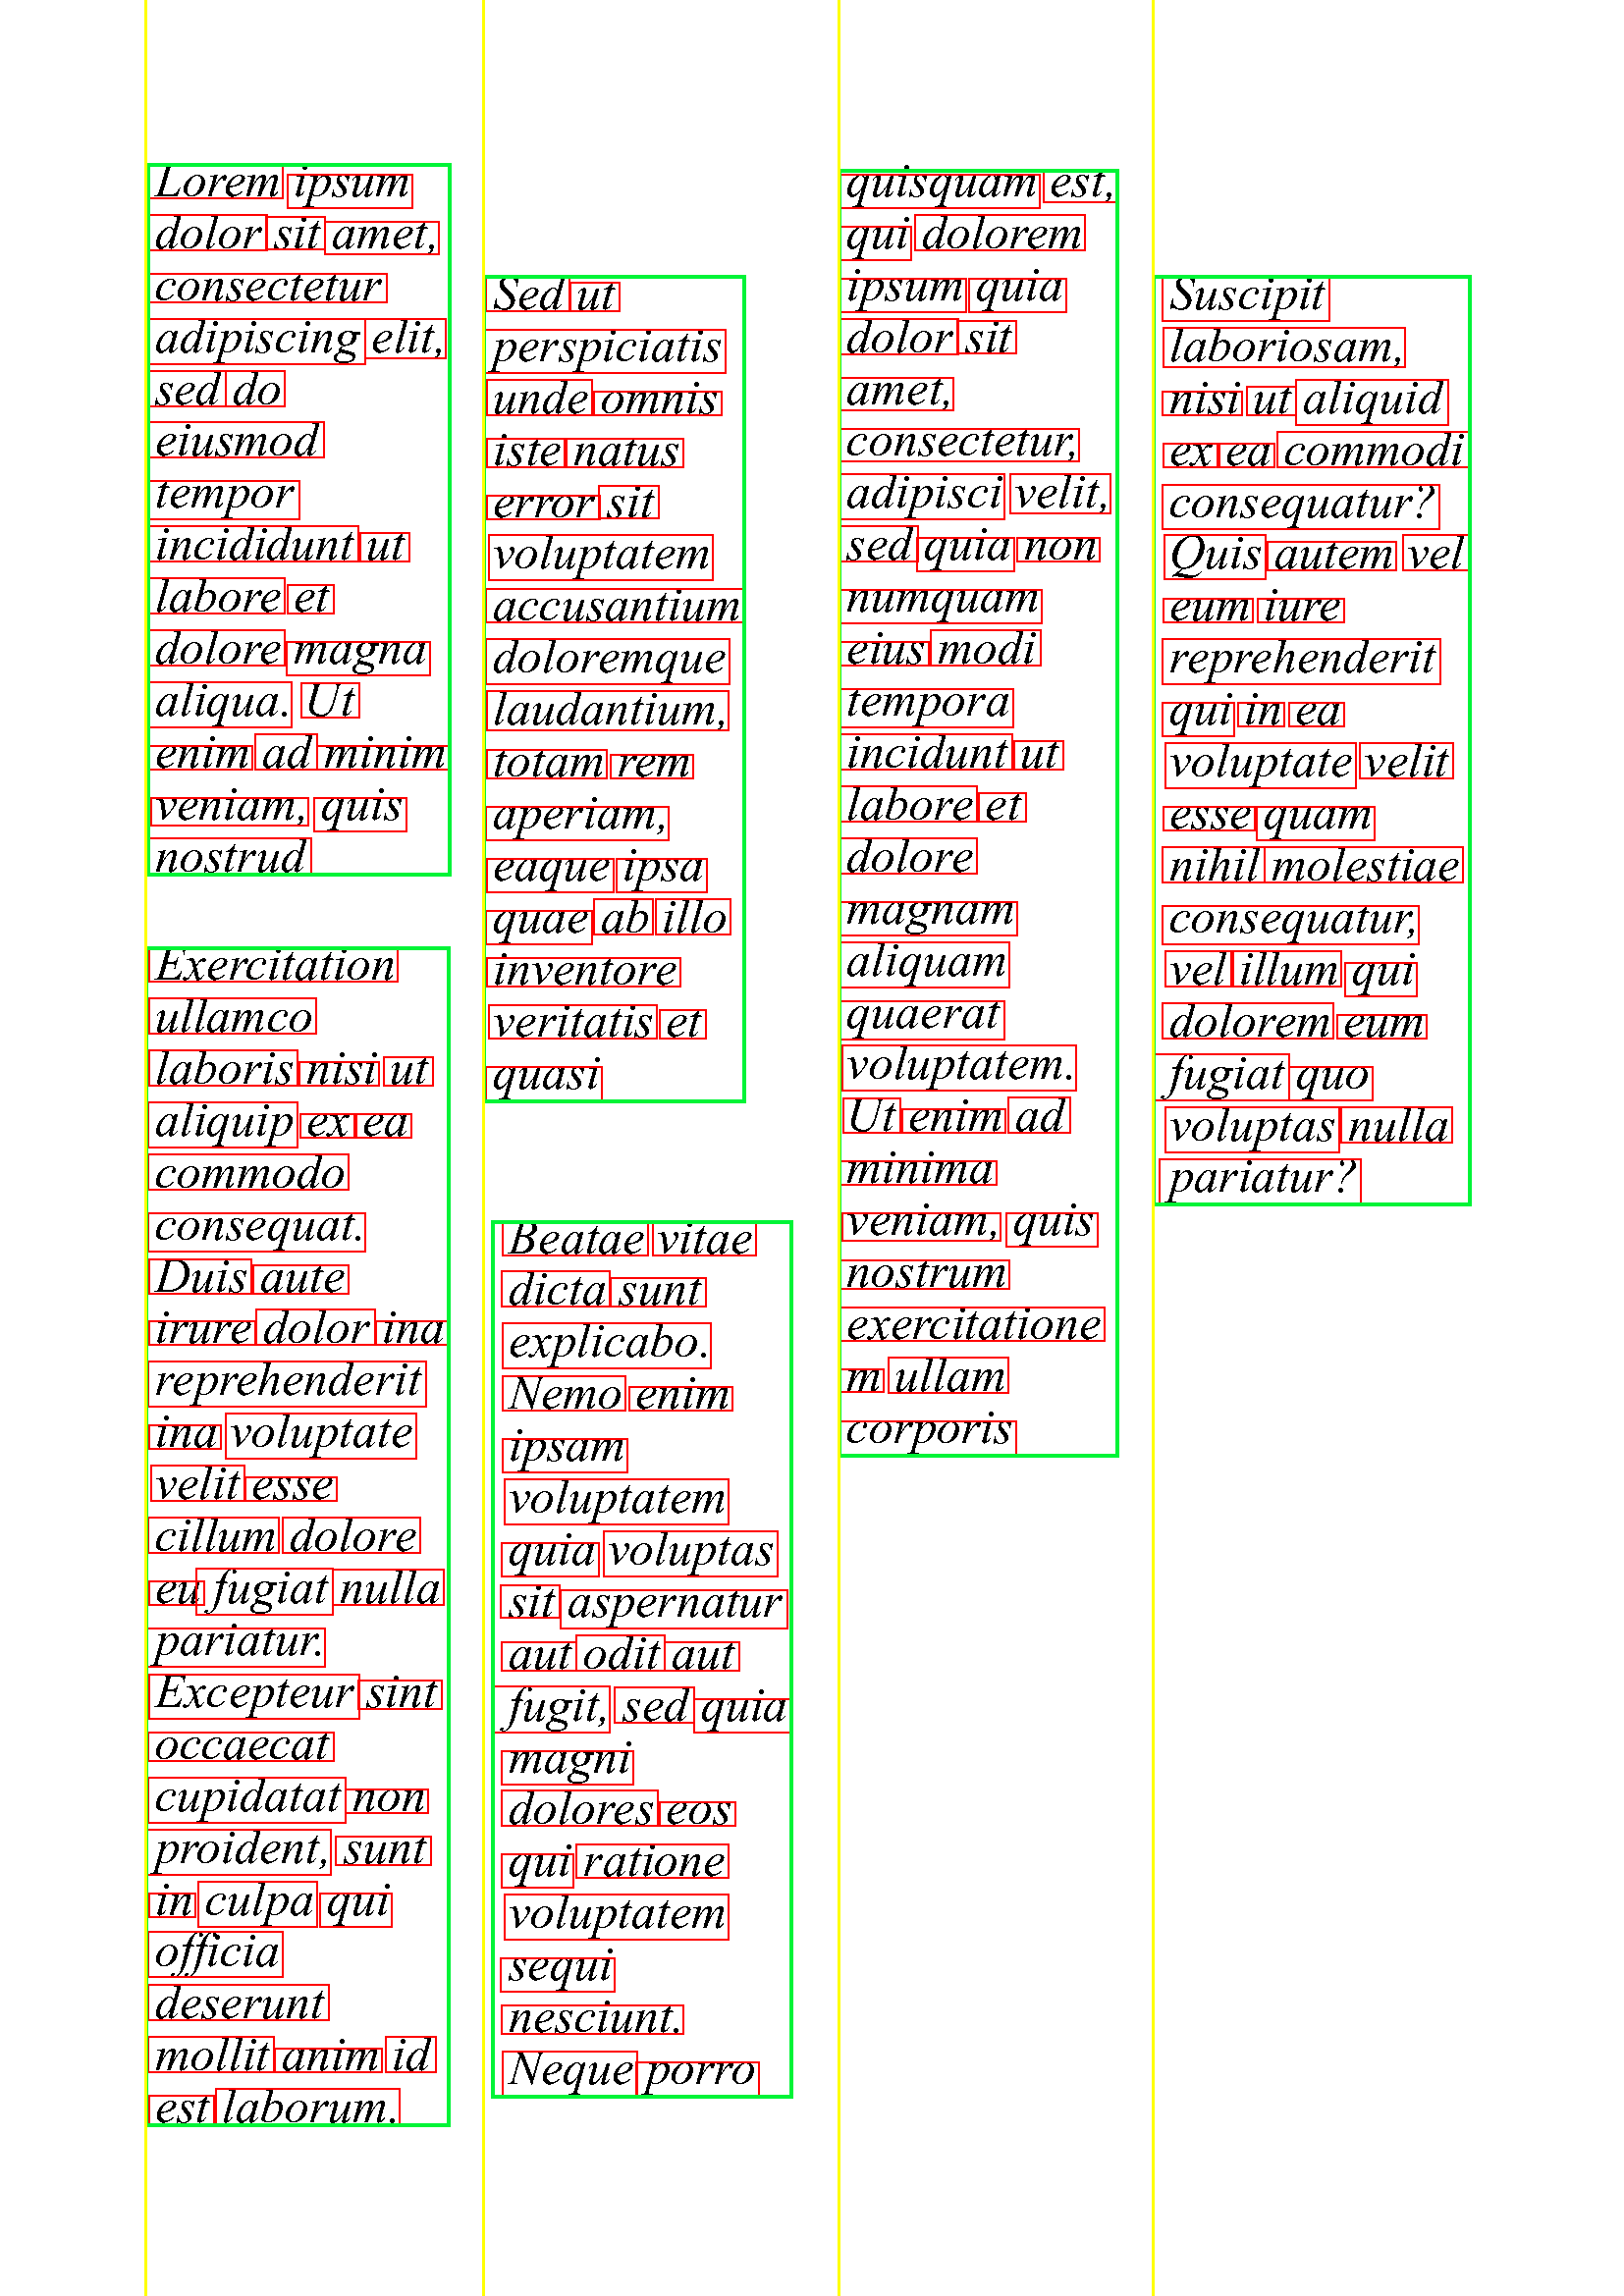
\includegraphics[scale=0.59]{./images/times_new_roman_colunas_4_blocos_6_linhas_38_palavras_197.png}
  \legend{ \small Fonte: Autor.}
\end{figure}


\begin{figure}[H]
  % impact_esquerda_tamanho_40_colunas_2_blocos_2_linhas_18_palavras_46
        \caption{\label{impact} \small Impact com tamanho 40, 2 colunas e 2 blocos de texto. }
        \begin{center}
            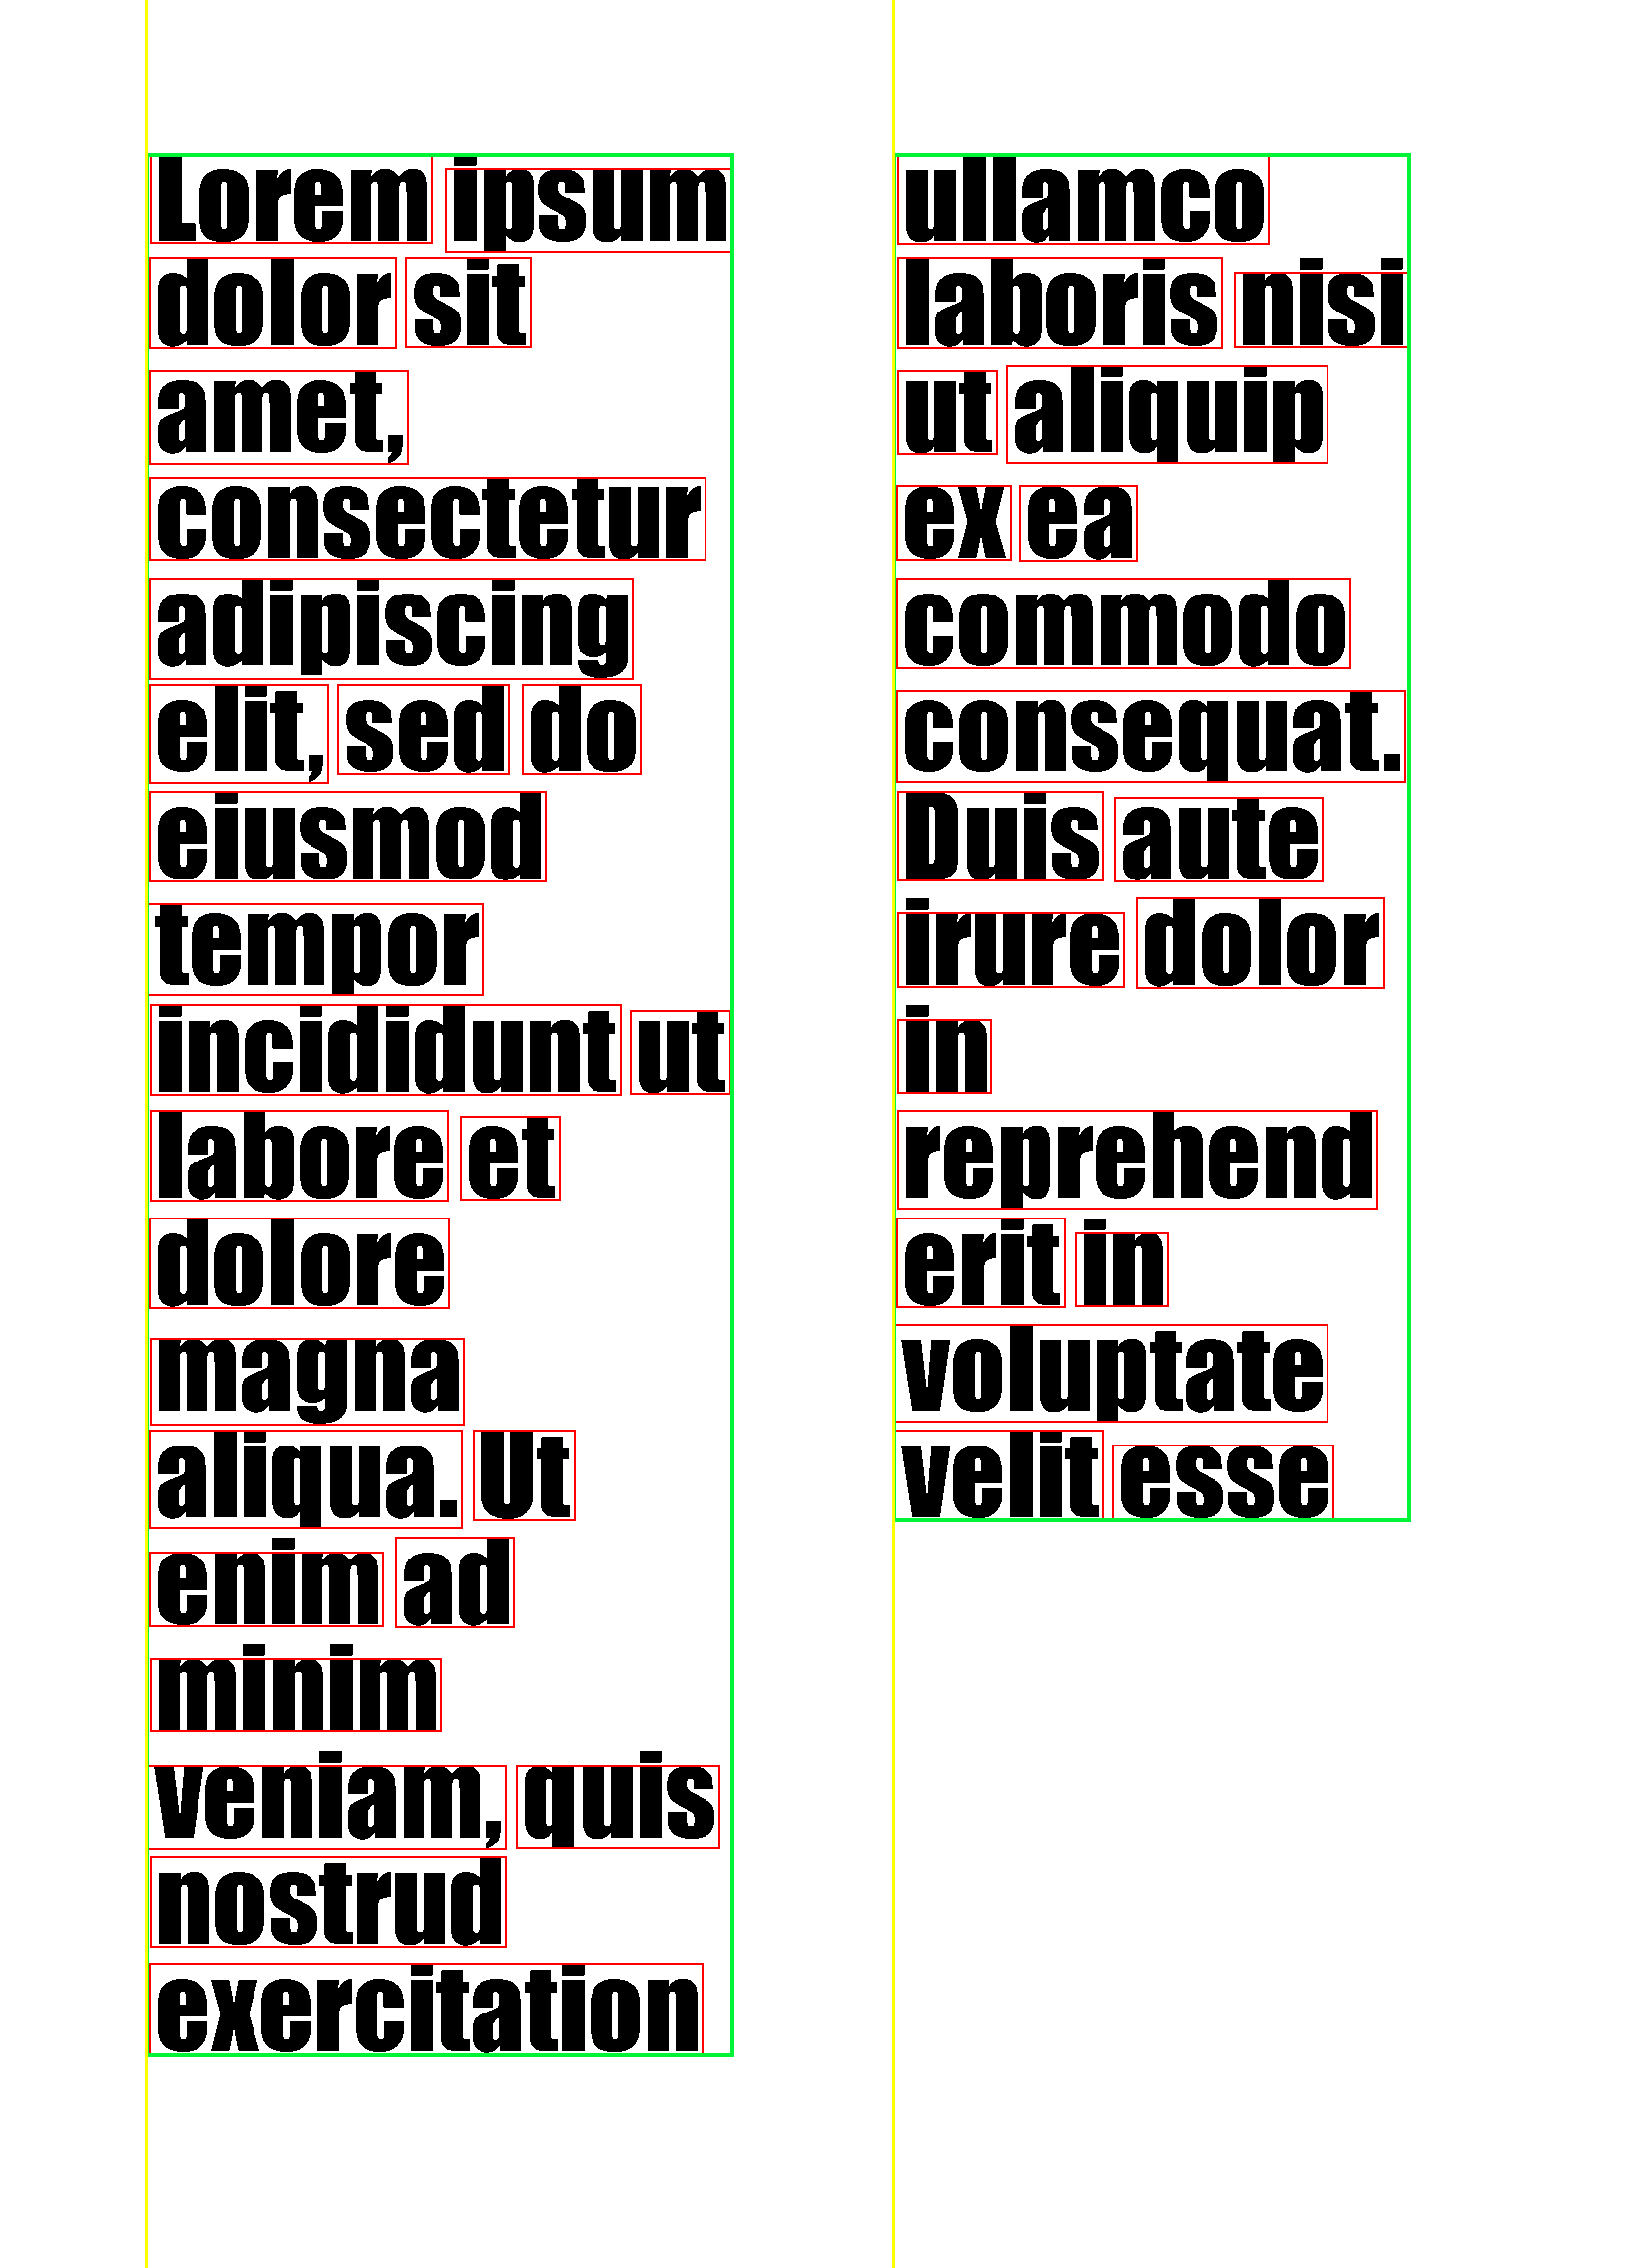
\includegraphics[scale=0.41]{./images/impact_columns.png}
        \end{center}
  \legend{ \small Fonte: Autor.}
\end{figure}

\begin{figure}[H]
        \caption{\label{arial} \small Arial justificado, com 12 de tamanho, 3 colunas e 8 blocos de texto.}
        \begin{center}
            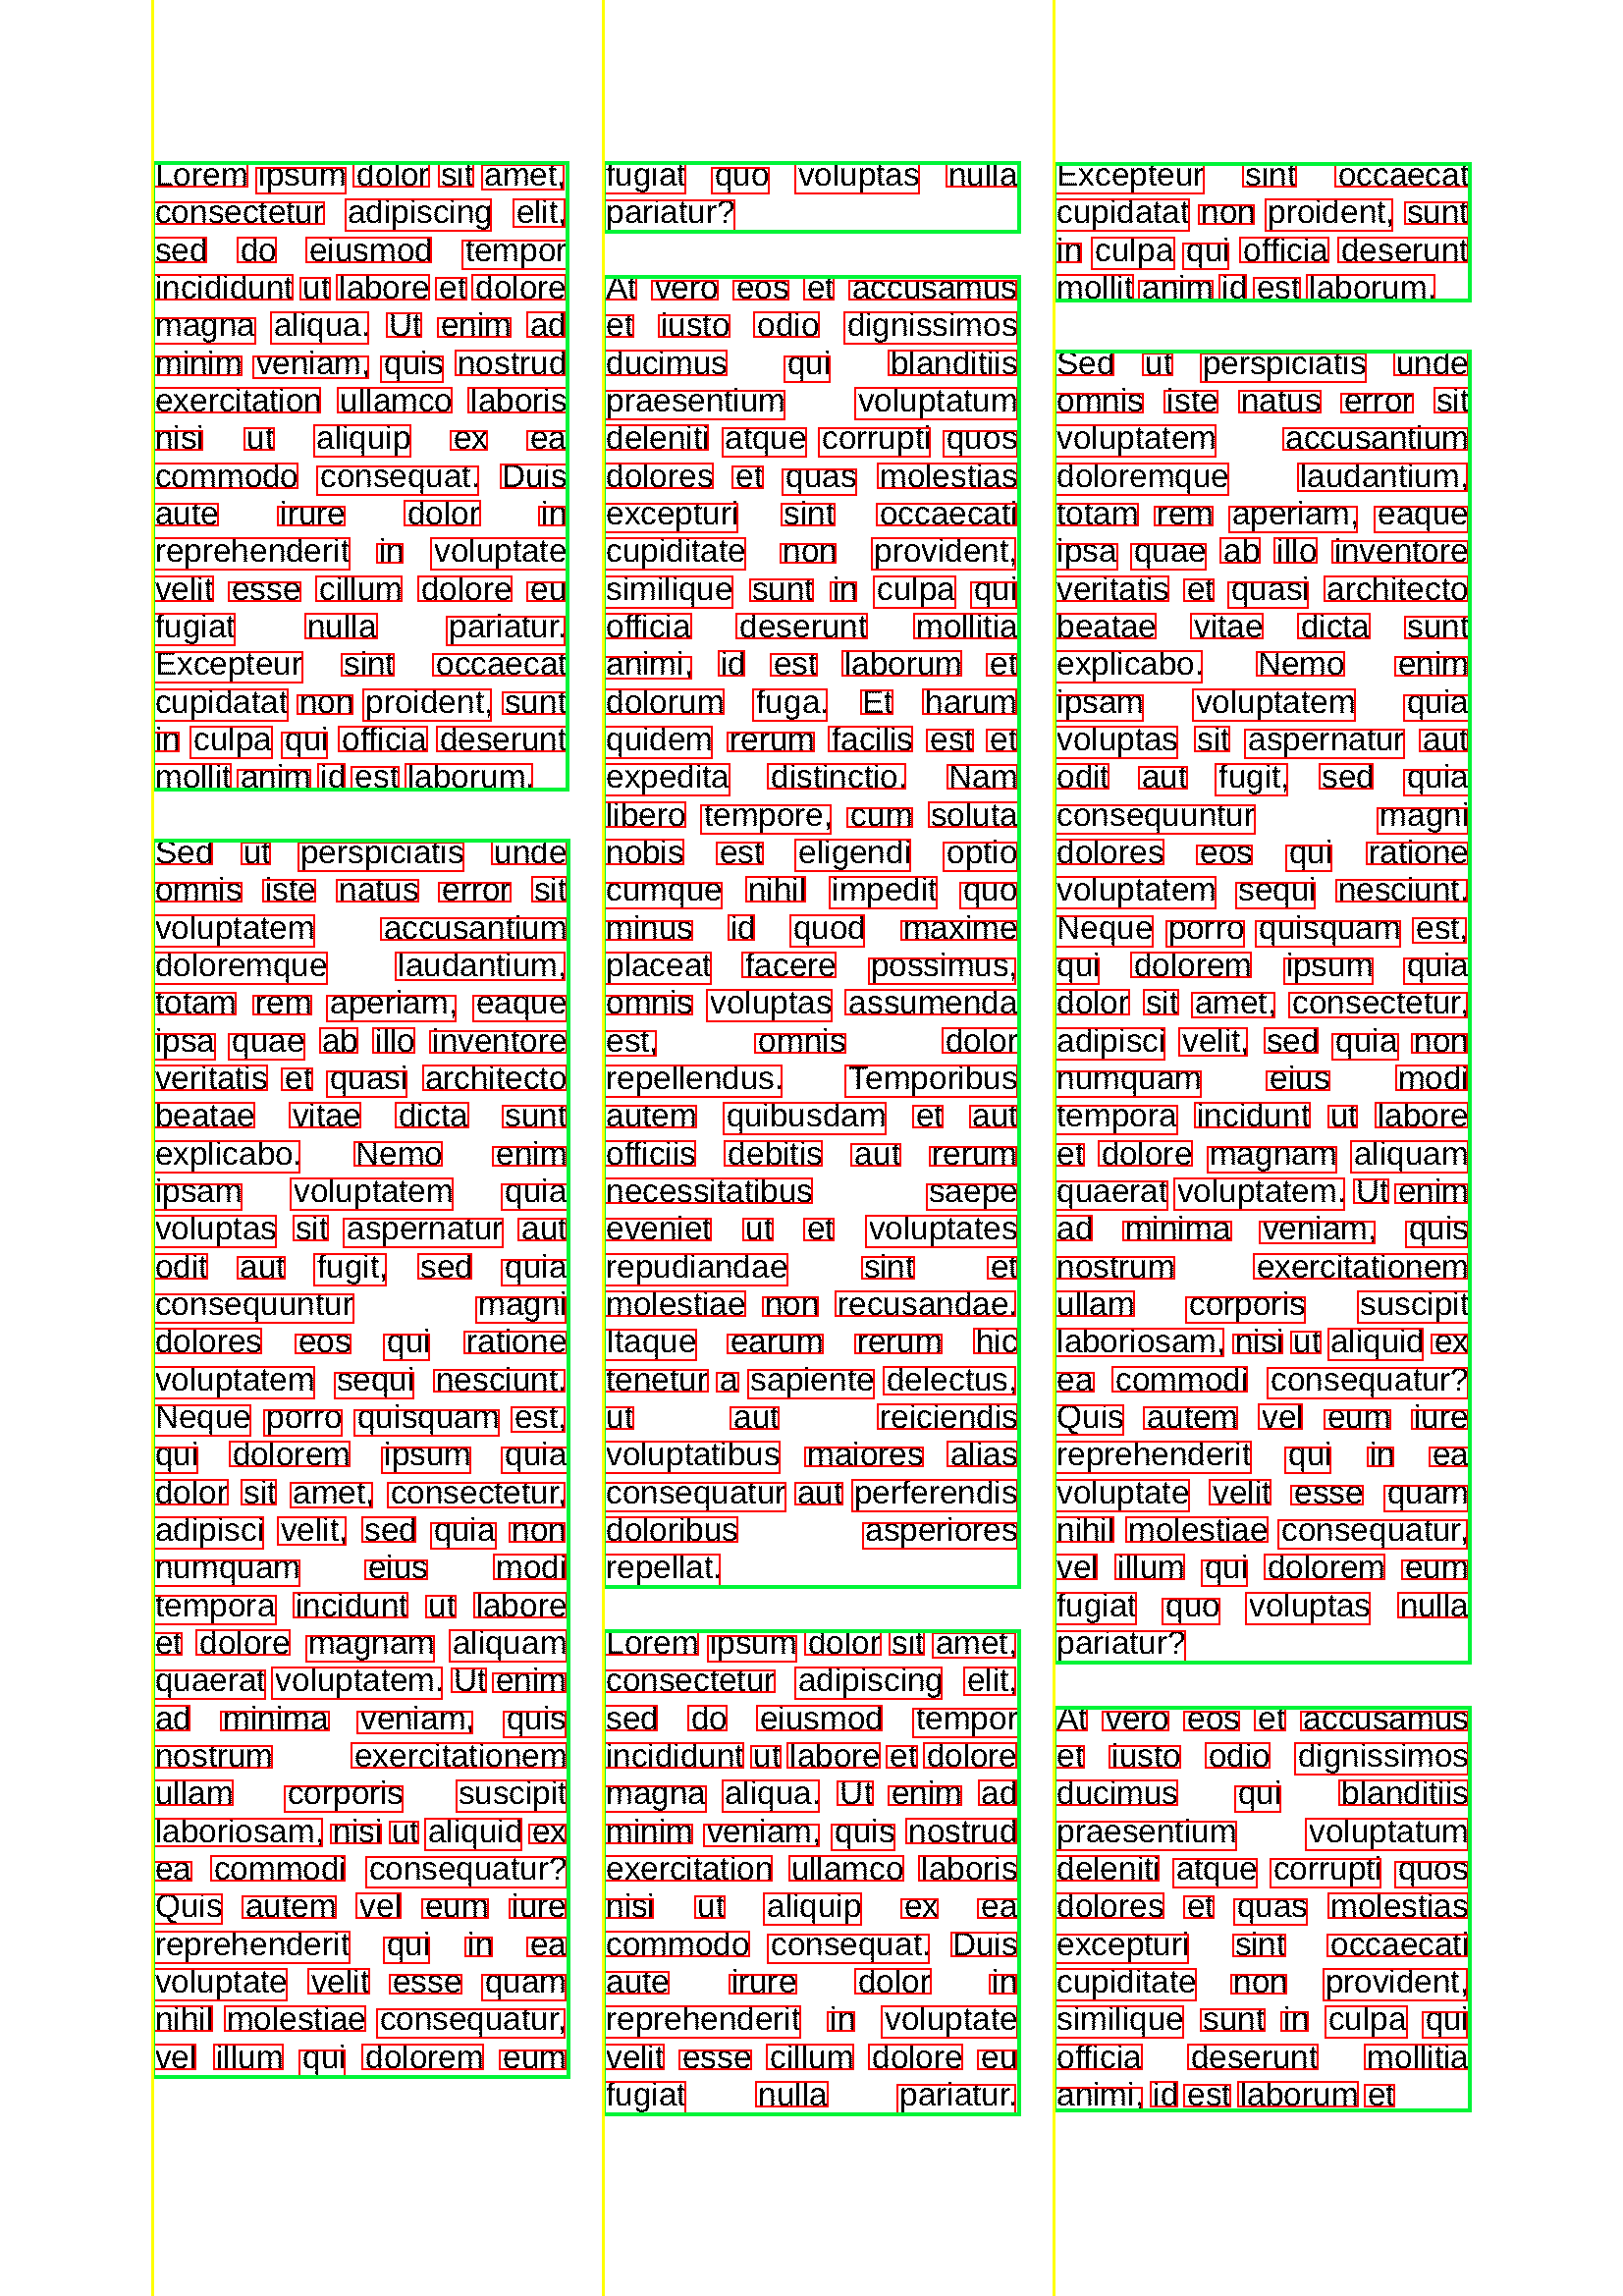
\includegraphics[scale=0.55]{./images/arial_justificado_tamanho_12_colunas_3_blocos_8_linhas_52_palavras_557.png}
        \end{center}
  \legend{ \small Fonte: Autor.}
\end{figure}


\section{Detalhes}

Inicialmente, o algoritmo lê a imagem de entrada e a pré-processa aplicando filtro da medianos (nome da função é no código \texttt{median\_blur}) e invertendo as cores. Essas etapas visam retirar possíveis ruídos do tipo sal de pimenta. O tamanho do filtro mediano é 3 de altura e largulo já que foi confirmado que os ruídos não passam do tamanho de 1 pixel. A inversão da imagem é feita para aplicar algoritmos morfológicos, como a dilatação, para melhorar a conectividade dos componentes de texto e facilitar o processamento subsequente. Dependendo dos parâmetros especificados, o algoritmo pode aplicar operações adicionais como fechamento (closing) ou abertura (opening) para refinar ainda mais as regiões de texto. A ideia é utilizar um elemento estruturante, conhecido como SE (do inglês, \textit{Structuring Element}), que connecte as letras; isso pode ser feito com um SE que seja horizontal. Foi testado com diferentes SEs, como fomarto circular, de cruz, vertical, mas o melhor é o horizontal. E faz sentido pois as letras vem logo à direta da anterior, então para conectalas, precisamos esticar na horizontal para "grudar" uma na outra. Veja como é da uma "esticada" para horzinhotal ao aplicar um SE [000] [111] [000].
\[
\begin{matrix}
0 & 0 & 0 \\
1 & 1 & 1 \\
0 & 0 & 0 \\
\end{matrix}
\]



Aplicação de operações de dilatação horizontal para melhorar a conectividade entre caracteres adjacentes.
Após as operações morfológicas, indetificamos as palavras individuais através componentes conectados dentro da imagem. Cada palavra é contida em uma bbox, que é desenhada retângulos ao redor delas na imagem de saída. Componentes conectados  é um conceito de grafos que pode ser aplicado numa imagem binarias, pixels brancos são nós. Existem tipos de connectividade. Se consideramos os vizinhos de um pixel como apenas esquerda, direita, cima e baixo, então temos 4-conectividade \cite[2.5.2 Adjacency, Connectivity, Regions, and Boundaries]{gonzalez2008digital}. Se adicionarmos as diagonais, agora temos 8-conectividade. O Algortimo para encontrar esses componentes conectados se basea numa busca profunda, marcado os visitados, toda vez que na imagem for não zero fazemos a busca até não encontrar mais caminhos, considerando as digonais. Se não encontramos mais caminhos quer dizer que esse é um compoenente. Repetimos até encontrar todos atualizando o ponto mais a em esquerda inferior e o maiis à direita superior do componente para encontrar o bbox da palavra. O código ilustra esse processo.


Também fazemos o agrupamento dessas palavras em blocos com base em sua proximidade espacial, possibilitando uma análise melhor da organização do texto podemos dizendo que cada bloco é um paragrafo.

Opcionalmente, aplicação de operações de fechamento e abertura para refinar as regiões de texto, dependendo dos parâmetros definidos.

Há uma dilatação adicional da imagem, se necessário, com base na altura média dos componentes de texto já filtrados.



Ao longo do processo, o algoritmo incorpora várias otimizações e ajustes de parâmetros para se adaptar a diferentes tipos de imagens de entrada e layouts de texto. Por exemplo, parâmetros como tamanho do kernel e contagens de iteração são ajustados dinamicamente com base nas características da imagem de entrada, como tamanho do texto e níveis de ruído.


Filtragem dos componentes de texto para eliminar bbox de pontuação e manter apenas bboxes de palavras.
Agrupamento de palavras em blocos com base em sua proximidade espacial.
Desenho de caixas delimitadoras ao redor das palavras e blocos identificados na imagem original.
Geração de um vídeo para visualizar interativamente as etapas do algoritmo.
Opcionalmente, escrita de imagens separadas para cada palavra identificada, para uso posterior em tentativas de reconhecimento óptico de caracteres (OCR).
Escrita da imagem final com caixas delimitadoras de palavras e blocos para análise adicional.

Além disso, o algoritmo fornece opções para gerar imagens intermediárias e vídeos para visualizar as etapas de processamento, auxiliando na depuração e compreensão do comportamento do algoritmo. Essas visualizações melhoram a transparência e a interpretabilidade da operação do algoritmo.

Em resumo, o algoritmo implementado demonstra uma abordagem abrangente para o reconhecimento de texto em imagens binárias, utilizando uma combinação de técnicas de processamento de imagem, regras heurísticas e parâmetros adaptativos. Ao refinar iterativamente regiões de texto e analisar seus relacionamentos espaciais, o algoritmo alcança uma detecção precisa de palavras, linhas, colunas e blocos, estabelecendo as bases para tarefas de reconhecimento de texto mais avançadas, como reconhecimento óptico de caracteres (OCR).

Ela é especialmente útil para preencher pequenos espaços ou quebrar conexões entre objetos. No \autoref{udilate} a função `understandable\_dilate` implementa função implementa uma dilatação morfológica de forma compreensível, percorrendo cada pixel da imagem.
A variável `kernel` representa o elemento estruturante, que define a forma e o tamanho da dilatação.
A imagem é percorrida pixel a pixel, e para cada pixel, verifica-se se pelo menos um dos pixels na vizinhança definida pelo kernel é branco (valor 255).
Se pelo menos um dos pixels na vizinhança é branco, o pixel central é definido como branco (255) na imagem resultante.
Caso contrário, o pixel central é definido como preto (0) na imagem resultante.
O parâmetro `iterations` indica quantas vezes a dilatação deve ser aplicada à imagem. Quanto maior o número de iterações, mais ampliado será o objeto na imagem.

\begin{codigo}[h]
  \caption{\small .}
 \label{udilate}
\begin{lstlisting}[language=python]
def understandable_dilate(image, kernel):
    result = np.zeros(image.shape)
    height = image.shape[0]
    width = image.shape[1]
    kernel_height = kernel.shape[1]
    kernel_width = kernel.shape[0]
    kernel_width_delta = kernel_width // 2
    kernel_height_delta = kernel_height // 2
    for y in range(height):
        for x in range(width):
            all_good = False
            for j in range(kernel_height):
                for i in range(kernel_width):
                    i_offset = i - kernel_width_delta
                    j_offset = j - kernel_height_delta
                    color = 0
                    if (
                        (x + i_offset) >= 0
                        and (x + i_offset) < width
                        and y + j_offset >= 0
                        and y + j_offset < height
                    ):
                        color = image[y + j_offset, x + i_offset]
                    kcolor = kernel[j, i]
                    if int(kcolor) * int(color):
                        all_good = True
                        break
                if all_good:
                    break
            if all_good:
                result[y, x] = 255
            else:
                result[y, x] = 0
    return result
\end{lstlisting}
\end{codigo}
    % Professora Bia, aqui eu disponho diferentes implementações de dilatação
    % understandable_dilate é o mais lento que tenta ser o mais entendivel possivel.
    % Ja fast_dilate2 é bem mais rapido, porém usa a função `maximum` da estrutura de dados matrix do  numpy.
    % é uma função que como o nome diz pega o maximo entre valores, mas funciona para matrix.
    % Eu dispus dessa maneira pra mostra que sei fazer todas as diferentes implementações,
    % mas pra ficar mais rapido e interativo é usado o fast_dilate2.
    % NOTE: Qualquer uma dessas implementações funciona para os propositos deste trabalho

Já no \autoref{fdilate2}, \texttt{fast\_dilate2} função implementa uma dilatação morfológica mais rápida, aproveitando as operações de matriz do NumPy. A imagem é expandida (padding) com um preenchimento adequado para evitar problemas de borda durante a aplicação (chamamos o SE de kernel no código). O SE é então aplicado à imagem usando a função `np.maximum`, que calcula o máximo elemento a elemento entre a image resultante e o subconjunto da imagem com padding. A imagem resultante começa com as entradas zero a medida que iteramos a altura $j$ e largura $i$ do SE, aplicamos essa função (maximum) num subconjunto diferente imagem com padding que depende do $j$ e $i$. Só aplicamos se o SE for maior igual à 1 na altura $j$ e largura $i$. Isso efetivamente realiza uma dilatação, onde o pixel central de uma vizinhança é definido como o valor máximo dessa vizinhança. Mas note que a vizinhaça depende do SE, apenas onde os valores são 1 é considerado visinhaça. Ambas as implementações alcançam o mesmo resultado de dilatação morfológica, mas a segunda função é mais eficiente computacionalmente devido ao uso de operações vetorizadas do NumPy. Isso resulta em uma execução mais rápida, especialmente em imagens grandes.

\begin{codigo}[h]
  \caption{\small.}
 \label{fdilate2}
\begin{lstlisting}[language=python]
def fast_dilate2(image, kernel):
    global counter 
    height, width = image.shape
    kernel_height, kernel_width = kernel.shape

    kernel_width_delta = kernel_width // 2
    kernel_height_delta = kernel_height // 2

    # We pad by the kernel delta, top, bottom, left and right
    padded_image = pad(
        image,
        kernel_height_delta,
        kernel_height_delta,
        kernel_width_delta,
        kernel_width_delta,
    )

    dilated = np.zeros(image.shape, dtype=np.uint8)
    for j in range(kernel_height):
        for i in range(kernel_width):
            if kernel[j, i] == 1:
                shifted_sub_image = padded_image[j : j + height, i : i + width]
                dilated = np.maximum(
                    dilated, shifted_sub_image
                )

    return dilated
\end{lstlisting}
\end{codigo}

Erosão segue a mesma ideia da dilação mas no caso a operação seria \texttt{minimum} no lugar de \textit{maximum} e a iteração começa com a imagem resultando com todas as entradas 1  no lugar de 0.  No caso da versão \texttt{understandable} da erosão, apenas quando todos os pixels das imagem alinhassem com o SE é que então é setado 1 no lugar de pelo menos um.  Note que erosão não é necessario para o projeto rodar bem, pois mesmo sem closing ou opening, o algoritmo é robusto para os casos de teste comentado na introdução. A função opening aplica a operação de abertura, que consiste em primeiro realizar uma erosão seguida de uma dilatação. É útil para remover pequenos ruídos e separar objetos próximos, mas nesse trabalho removemos pelo filtro da mediana. Além disso buscamos juntar e não separar objetos, então opening é só usando após um closing para controlar a dilatação.

\begin{codigo}[h]
  \caption{\small.}
 \label{fdilate2}
\begin{lstlisting}[language=python]
def fast_dilate2(image, kernel):
    global counter 
    height, width = image.shape
    kernel_height, kernel_width = kernel.shape

    kernel_width_delta = kernel_width // 2
    kernel_height_delta = kernel_height // 2

    # We pad by the kernel delta, top, bottom, left and right
    padded_image = pad(
        image,
        kernel_height_delta,
        kernel_height_delta,
        kernel_width_delta,
        kernel_width_delta,
    )

    dilated = np.zeros(image.shape, dtype=np.uint8)
    for j in range(kernel_height):
        for i in range(kernel_width):
            if kernel[j, i] == 1:
                shifted_sub_image = padded_image[j : j + height, i : i + width]
                dilated = np.maximum(
                    dilated, shifted_sub_image
                )

    return dilated
\end{lstlisting}
\end{codigo}


A contagem de linhas proposto baseia-se na análise de das bboxes que cercam as regiões de texto.
Primeiro verifica se a lista de caixas delimitadoras está vazia. As caixas são ordenadas verticalmente com base na coordenada y. Para cada caixa, calcula-se a sobreposição vertical com a caixa anterior. Se a sobreposição for menor que uma fração mínima, a caixa é contada como uma nova linha. A cada interação criamos uma imagem intermediaria para geração do video, nele exibimos as bboxes realçando corretamente as linhas de texto.

O algoritmo para contar colunas é similar ao de linhas, mas agora ordenamos pelo horizontal no lugar da vertical.
Mantemos uma variavel para contar o número de colunas e max\_right para acompanhar a coordenada x do canto inferior direito da caixa mais à direita encontrada até o momento.

Para cada caixa delimitadora ordenada, verifica-se se sua coordenada x do canto inferior esquerdo é maior do que a coordenada x do canto inferior direito da caixa mais à direita encontrada até o momento (max\_right). Se for, considera-se isso como o início de uma nova coluna e incrementa-se o contador de colunas (num\_columns). Também é desenhada uma linha vertical indicando o início da nova coluna na imagem de vídeo.

A coordenada x do canto inferior direito da caixa mais à direita (max\_right) é atualizada, se necessário.

No final, a imagem de vídeo atualizada é adicionada à lista video\_frames para visualização posterior, e o número total de colunas encontradas é retornado (num\_columns).


Para agrupar os paragrafos ou blocos A função começa inicializando uma lista vazia chamada result para armazenar os grupos de caixas delimitadoras agrupadas.

Em seguida, inicializa uma lista chamada rest\_idxs que contém os índices de todas as caixas delimitadoras não agrupadas inicialmente.

Enquanto ainda houver índices na lista rest\_idxs, o algoritmo continua a iterar:

Ele retira um índice da lista rest\_idxs e o adiciona à lista close\_idxs, que representa o grupo de caixas delimitadoras próximas.

Em seguida, calcula a distância entre a caixa delimitadora selecionada (bbox) e todas as outras caixas delimitadoras não agrupadas. Se a distância entre duas caixas delimitadoras for menor do que a max\_distance especificada ou se houver uma sobreposição significativa entre elas, as duas caixas são consideradas próximas o suficiente para serem agrupadas.

Se uma caixa delimitadora for adicionada ao grupo, ela é removida da lista rest\_idxs, e a função recalcula a caixa delimitadora que envolve todas as caixas no grupo atualizado.

Durante esse processo, a função também desenha retângulos em uma imagem de vídeo (representada por image) para visualização. Cada retângulo delimita o agrupamento de caixas delimitadoras.

Após a conclusão do processo de agrupamento para um determinado grupo de caixas delimitadoras próximas, o grupo resultante é adicionado à lista result.

Finalmente, a função retorna a lista result, que contém todos os grupos de caixas delimitadoras agrupadas com base na distância máxima especificada.







\begin{codigo}[h]
  \caption{\small.}
 \label{group_bboxes}
\begin{lstlisting}[language=python]
def group_bboxes(bboxes, max_distance, image) -> list[list]:
    """
    Group bboxes based on a max distance.
    `image` is video for purposes
    """
    result = list()
    rest_idxs = [i for i in range(len(bboxes))]
    while len(rest_idxs) > 0:
        close_idxs = [rest_idxs.pop()]
        bbox = bboxes[close_idxs[0]]
        counter = 0
        while counter < len(rest_idxs):
            r_idx = rest_idxs[counter]
            counter += 1
            dist = distance(bbox, bboxes[r_idx])
            if (dist < max_distance) or bbox_overlap(bbox, bboxes[r_idx]):
                close_idxs.append(r_idx)
                rest_idxs.remove(r_idx)
                bbox = enclosing_bbox([bbox, bboxes[r_idx]])
                counter = 0

                vid_img = image.copy()
                y, x, y2, x2 = bbox
                rectangle(vid_img, (y, x), (y2, x2), (0, 244, 55), 2)
                video_frames.append(vid_img)

        y, x, y2, x2 = bbox
        rectangle(image, (y, x), (y2, x2), (0, 244, 55), 2)
        result.append([bboxes[i] for i in close_idxs])
    return result
\end{lstlisting}
\end{codigo}

A função começa definindo os vizinhos possíveis para o algoritmo de busca em profundidade (DFS, na sigla em inglês). Dependendo do parâmetro de conectividade, pode haver 4 ou 8 vizinhos possíveis. Os vizinhos são definidos como deslocamentos na grade, representando movimentos para cima, para baixo, para a esquerda e para a direita. Se a conectividade for 8, são adicionados deslocamentos diagonais também.

Em seguida, a função define uma função interna chamada dfs, que realiza a busca em profundidade. Esta função recebe as coordenadas (y, x) de um ponto inicial na imagem e explora recursivamente todos os pixels conectados a esse ponto.

O dfs mantém uma pilha de pixels a serem visitados. Ele começa visitando o ponto inicial (y, x) e verifica se ele está dentro dos limites da imagem, se não foi visitado anteriormente e se é um pixel branco (valor 255).

Se o pixel atual satisfizer todas essas condições, ele é marcado como visitado, e as coordenadas mínimas e máximas da caixa delimitadora ao redor deste componente conectado são atualizadas.

Depois, o algoritmo verifica os vizinhos do pixel atual, adicionando-os à pilha de pixels a serem visitados.

O algoritmo continua explorando todos os pixels conectados até que não haja mais pixels na pilha.

Após explorar completamente um componente conectado, a função dfs retorna as coordenadas mínimas e máximas da caixa delimitadora que envolve esse componente.

A função principal inicializa uma matriz booleana visited para rastrear quais pixels já foram visitados durante a exploração dos componentes conectados.

Então, percorre todos os pixels da imagem e, para cada pixel branco não visitado, chama a função dfs para explorar o componente conectado a esse pixel.

Por fim, as coordenadas mínimas e máximas de cada componente conectado são adicionadas a uma lista de caixas delimitadoras, que é retornada como o resultado final da função.
\begin{codigo}[h]
  \caption{\small.}
 \label{fdilate2}
\begin{lstlisting}[language=python]
def find_connected_components_bboxes(image, min_area=0, connectivity=8):
    nbrs = [(1, 0), (-1, 0), (0, 1), (0, -1)]
    if connectivity == 8:
        nbrs.extend([(1, 1), (1, -1), (-1, 1), (-1, -1)])

    def dfs(y, x):
        nonlocal nbrs, image
        min_y, min_x, max_x, max_y = y, x, y, x
        stack = [(y, x)]
        while stack != list():
            cy, cx = stack.pop()
            if (
                0 <= cy < image.shape[0]
                and 0 <= cx < image.shape[1]
                and not visited[cy, cx]
                and image[cy, cx] == 255
            ):
                visited[cy, cx] = True
                min_y = min(min_y, cy)
                min_x = min(min_x, cx)
                max_x = max(max_x, cy)
                max_y = max(max_y, cx)

                for dy, dx in nbrs:
                    stack.append((cy + dy, cx + dx))
        return min_y, min_x, max_x, max_y

    visited = np.zeros(image.shape, dtype=bool)
    bounding_boxes = list()

    for y in range(image.shape[0]):
        for x in range(image.shape[1]):
            if not visited[y, x] and image[y, x] == 255:
                min_y, min_x, max_x, max_y = dfs(y, x)
                bounding_boxes.append((min_y, min_x, max_x, max_y))

    return bounding_boxes

\end{lstlisting}
\end{codigo}





% Breve descrição do problema abordado no trabalho.
% Objetivo do trabalho.
% Descrição do Problema:

% Explicação detalhada do problema proposto.
% Especificações da entrada e saída do programa.
% Exemplos\chapter{M de imagens de entrada e saída.

\chapter{Estrutura do Projeto}

\chapter{Requisitos}

\begin{verbatim}
python3 src/main.py assets/grupo_13_arial_esquerda_tamanho_16_colunas_2_blocos_4_linhas_39_palavras_318.pbm
\end{verbatim}



\chapter{Métodos e Implementações}

% Descrição das técnicas utilizadas para resolver o problema.
% Explicação de como as técnicas aprendidas na disciplina foram aplicadas.
% Parâmetros utilizados durante o processamento das imagens.

% Implementação:
% Inclusão de código-fonte relevante ou detalhes adicionais sobre a implementação, se necessário.
Seguindo as formulas de dilatação em \cite[capitulo 9]{gonzalez2008digital}

\chapter{Resultados}

implementção \url{https://www.youtube.com/watch?v=uA45GeodGss}
Descrição da implementação do programa.
Destaque para soluções desenvolvidas para problemas específicos encontrados durante o desenvolvimento.
Resultados:

Apresentação dos resultados obtidos.
Inclusão de exemplos de imagens de entrada e saída.
Discussão sobre a eficácia do programa e eventuais limitações.


\chapter{Conclusão}

Sumarização dos principais resultados e contribuições do trabalho.
Reflexão sobre o aprendizado durante o desenvolvimento do programa.
Sugestões para trabalhos futuros ou melhorias no programa.




\phantompart
\bibliography{Bibliografia}


%%%%%%%%%%%%%%%%%%%%%%%%%%%%%%%%%%%%%%%%%%%%%%%%%%%%%%
% ELEMENTOS PÓS-TEXTUAIS
%%%%%%%%%%%%%%%%%%%%%%%%%%%%%%%%%%%%%%%%%%%%%%%%%%%%%%


\postextual


\renewcommand{\chapnumfont}{\chaptitlefont}
\renewcommand{\afterchapternum}{}
% \include{Pos_Textual/Apendices}
% \include{Pos_Textual/Anexos}


\end{document}
